% Created 2017-04-05 mié 00:18
% Intended LaTeX compiler: pdflatex
\documentclass[11pt]{/home/hao/dev/org/latex-plantilla/IEEEtran}
\usepackage[spanish, mexico]{babel}
\usepackage{url}
\usepackage{minted}
\addto\captionsspanish{\renewcommand{\contentsname}{Contenido}}
\usepackage[utf8]{inputenc}
\usepackage[T1]{fontenc}
\usepackage{graphicx}
\usepackage{grffile}
\usepackage{longtable}
\usepackage{wrapfig}
\usepackage{rotating}
\usepackage[normalem]{ulem}
\usepackage{amsmath}
\usepackage{textcomp}
\usepackage{amssymb}
\usepackage{capt-of}
\usepackage{hyperref}
\author{Eduardo Vázquez Díaz \\ lalohao@gmail.com}
\date{\today}
\title{Verificación de circuitos digitales con software libre}
\hypersetup{
 pdfauthor={Eduardo Vázquez Díaz \\ lalohao@gmail.com},
 pdftitle={Verificación de circuitos digitales con software libre},
 pdfkeywords={},
 pdfsubject={},
 pdfcreator={Emacs 25.1.1 (Org mode 9.0.5)},
 pdflang={Spanish}}
\begin{document}

\maketitle
\tableofcontents

\begin{abstract}
Se creó una maquina virtual con \emph{Ubuntu Desktop 16.04.1} \uline{LTS} en un
contenedor utilizando el software de virtualizacion \texttt{Qemu}, donde
posteriormente se instaló \texttt{verilator} y \texttt{gtkwave}; a partir de este
sistema se exponen algunas técnicas para simular circuitos con
verilog/C++, además de visualizar las ondas generadas de manera
gráfica.
\end{abstract}

\section{Introducción}
\label{sec:org5f51a6c}
La importancia de probar los circuitos antes de ser llevados al
silicio puede representar millones de dolares, sin contar el tiempo
invertido en el diseño, y el que se necesitará volver a invertir
para arreglarlo.

En 1990 el lenguaje de descripción de hardware mas usado era VHDL a
pesar de que solo tenia constructores básicos para probar
(TestBench) los circuitos. Los diseños empezaban a crecer y nuevo
software comercial se creaba para compensar la falta de funciones.
Algunas empresas invertían horas de trabajo para crear su propio
sistema y no pagar los miles de dolares en licencias, una de ellas
llevó a la creación de Accelera que fue la base de SystemVerilog
\cite{spear08_system}.

De la misma manera surgió \texttt{Verilator}, un simulador potente de
Verilog HDL que además es software libre, este compila el código y
lo optimiza para ser simulado rápidamente \cite{verilator-intro}, en
algunos casos es incluso mas veloz que los simuladores comerciales
\cite{verilator-vs-comercial}.

\subsection{Virtualización}
\label{sec:org111b7e3}
La maquina virtual permite encapsular el sistema de verificación de
circuitos en un contenedor que no será afectado (y que no afectará)
la maquina utilizada, esto elimina errores que podrian ser causados
al tener instalado software que utilice configuraciones con
variables globales (PATHS) como ocurre con \texttt{HSPICE} y \texttt{Questa SIM}
por ejemplo.

\begin{center}
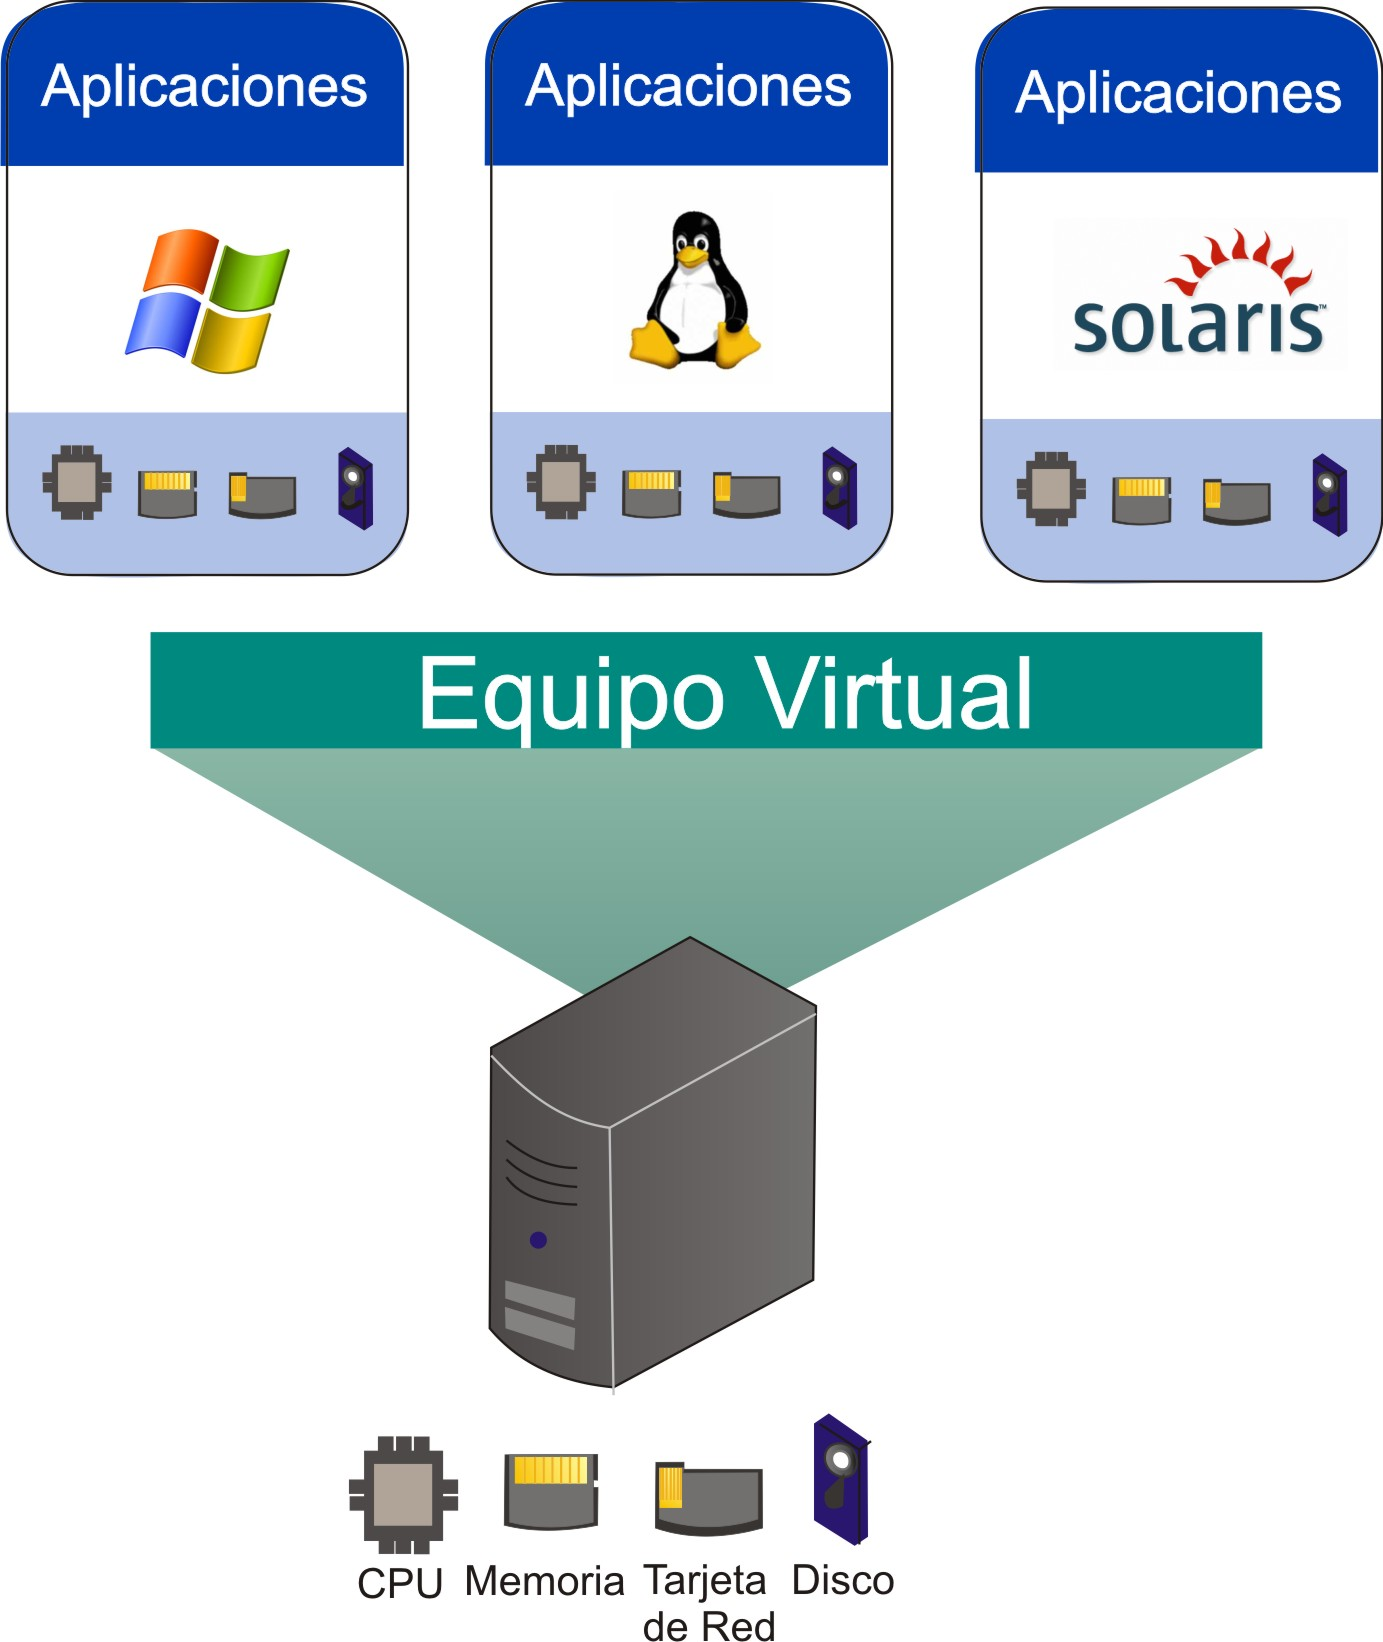
\includegraphics[width=7cm]{virtualizacion.jpg}
\captionof{figure}{\label{fig:org1ca3eb9}
Las maquinas virtuales pueden o no conectarse entre ellas o hacia la red externa y pueden ser de diferentes arquitecturas y sistemas operativos independientemente del sistema anfitrion.}
\end{center}

Se le dice anfitrión a la maquina donde se encuentran los
contenedores virtuales, en este caso la anfitriona usa \emph{Arch
Linux}, pero esto no afecta a los contenedores ya que estan
aislados, por lo que esto se puede aplicar de igual manera en
Windows o Mac.
\section{Desarrollo}
\label{sec:org7edc0b0}
Para instalar la maquina virtual se utiliza la linea de comandos,
creando el disco duro virtual llamado \textbf{verif}, con un tamaño de
10Gb, posteriormente se carga el archivo \texttt{ISO} de Ubuntu en el disco
duro creado, con 2G de memoria RAM y se procede a instalar el
sistema operativo de forma normal.

\begin{minted}[]{bash}
qemu-img create -f raw verif 10G
qemu-system-x86_64 -cdrom ubuntu.iso \
                   --boot order=d -drive \
                   file=verif,format=raw \
                   -m 2G
\end{minted}

Una vez instalado el sistema operativo se puede iniciar de la
siguiente forma:

\begin{minted}[]{bash}
qemu-system-x86_64 --boot order=d \
   -drive file=verif,format=raw -m 2G
\end{minted}

Posteriormente en la maquina virtual (Ubuntu) se instala el software
necesario para simular \cite{verilator-instalacion}, al igual que el
editor de texto de su preferencia para modificar los archivos :

\begin{minted}[]{bash}
sudo apt-get install git make \
     autoconf g++ flex bison \
     verilator gtkwave
\end{minted}
\subsection{Ejemplo 1: Compuerta AND}
\label{sec:org8721df7}
Para entender el proceso de simulación es necesario entender la
estructura jerárquica del espacio de trabajo.

Clona el siguiente repositorio:

\begin{minted}[]{shell}
git clone \
github.com/LaloHao/verilator_test
\end{minted}

Dentro se encuentra una carpeta donde se simula la compuerta \texttt{and},
en ella se encuentran los siguientes archivos:

\begin{minted}[]{bash}
cand_tb.cpp
cand.v
cand.vcd
Makefile
README.md
\end{minted}

El archivo \texttt{README} se puede ignorar; los archivos donde se
describe el comportamiento y el testbench son \textbf{cand.v},
\textbf{cand-tb.cpp} respectivamente, después se encuentra el archivo
\textbf{cand.vcd} que es utilizado por el programa \texttt{gtkwave} para
visualizar las ondas al simularse, por ultimo el archivo \textbf{Makefile}
donde contienen todos los comandos necesarios para ejecutar y abrir
el visor de ondas.

Dentro de la carpeta \emph{and} al ejecutar el comando \texttt{make} se
simulará, ejecutará, y abrirá el visor de ondas automáticamente.

\begin{center}
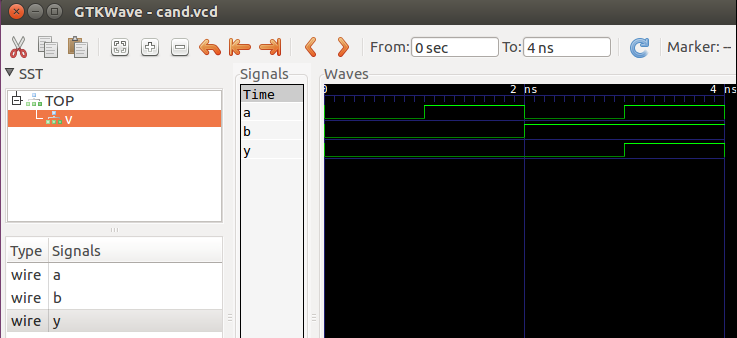
\includegraphics[width=9cm]{data/51/264eef-d888-4bbb-933e-983c0be58cb7/screenshot-20170217-105525.png}
\captionof{figure}{\label{fig:org06f0a1d}
Visor de ondas mostrando la simulacion de la compuerta \texttt{and}.}
\end{center}

El archivo con extensión \textbf{.v} describe el comportamiento del
circuito como ya se mencionó, estas son sentencias Verilog
pertinentes al lenguaje por lo que se omite la explicación de su
contenido.

\subsubsection{Testbench}
\label{sec:org051699d}
El archivo de testbench (extensión \textbf{.cpp}) contiene las
instrucciones necesarias para simular.

Al ejecutarse el comando \texttt{make} Verilator genera los archivos
\textbf{Vcand.cpp} y \textbf{Vcand.h} dentro de una carpeta llamada \emph{obj\(_{\text{dir}}\)}
donde se contienen funciones que son llamadas para controlar el
flujo de señales y agregarlas al archivo \textbf{.vcd} donde se
visualizaran, por ello es necesario incluirlo para referenciarlas
desde el testbench al igual que los \emph{headers} de Verilator:

\begin{minted}[]{cpp}
#include "Vcand.h"
#include "verilated.h"
#include "verilated_vcd_c.h"
\end{minted}

Dentro del testbench se crea un pulso de reloj que se utiliza como
referencia para controlar el tiempo que correrá la simulación.

\begin{minted}[]{cpp}
int clk;
\end{minted}

Las siguientes lineas son para Verilator exceptuando las que
contienen referencias a \textbf{Vcand} y \textbf{VcdC}; \textbf{Vcand} instancia el
objeto \textbf{cand.v} el cual se incluyó anteriormente, \textbf{Vcdc} es la
instancia del objeto donde se guardarán las ondas para
visualizacion.

\begin{minted}[]{cpp}
Verilated::commandArgs(argc, argv);
Vcand *top = new Vcand;
Verilated::traceEverOn(true);
VerilatedVcdC *tfp = new VerilatedVcdC;
\end{minted}

El objeto llamado \textbf{top} es el archivo \textbf{cand.v}, desde ahí se
pueden inicializar y modificar las señales, de igual el objeto
\textbf{tfp} define en que archivo se guardarán las ondas, se enlazan por
medio de \texttt{trace}:

\begin{minted}[]{cpp}
top->trace(tfp, 99);
tfp->open("cand.vcd");
top->a = 0;
top->b = 0;
\end{minted}

Se usa un ciclo y envían todas las señales posibles usando
\texttt{dump} para volcar las señales al archivo:

\begin{minted}[]{cpp}
for(clk = 0; clk <= 4; clk++)
{
    tfp->dump(clk);
    top->a = !top->a;
    top->b = (clk >= 1);
    top->eval();
}
\end{minted}

Finalmente se dan las instrucciones pertinentes a Verilator para
terminar la simulación:

\begin{minted}[]{cpp}
if(Verilated::gotFinish())
    exit(0);
tfp->close();
exit(0);
\end{minted}

Los nombres descriptivos de variables facilitan el reconocimiento
de cada objeto en proyectos mas grandes, como se verá en el
siguiente ejemplo.
\subsection{Ejemplo 2: Memoria RAM}
\label{sec:orgc6cafb4}

Clona el repositorio:

\begin{minted}[]{shell}
git clone \
github.com/LaloHao/8bit-cpu
\end{minted}

En el se encuentran un diseño de una memoria RAM y un CPU (\hyperref[sec:org105a531]{Ejemplo 3: CPU}).

\begin{minted}[]{shell}
cpu.v
cpu_tb.v
ram.v
ram_tb.v
\end{minted}
\subsubsection{Testbench}
\label{sec:orgdfb1dce}
El archivo \textbf{ram\(_{\text{tb.v}}\)} contiene el testbench, algunos nombres de
variables se han cambiado para dar mas claridad, por ejemplo:

\begin{minted}[]{cpp}
VerilatedVcdC * gtkw = new VerilatedVcdC;
Vram *ram = new Vram;
ram->trace(gtkw, 99);
gtkw->open("ram.vcd");
\end{minted}

Recordando que al estar usando un lenguaje como C++ se tiene todos
sus operadores:

\begin{minted}[]{cpp}
#define WRITE 1
#define READ 0
\end{minted}

Permitiendo definir la operación que realiza la RAM:

\begin{minted}[]{cpp}
ram->rw = WRITE;
ram->rw = READ;
\end{minted}
\begin{enumerate}
\item Escritura
\label{sec:org5088d85}
\begin{center}
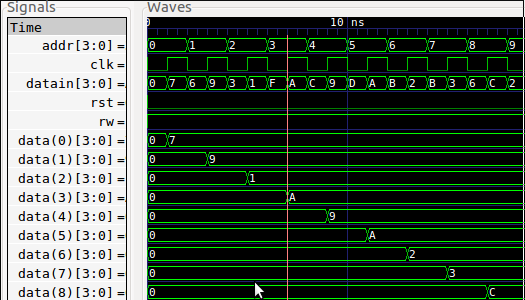
\includegraphics[width=9cm]{data/6d/c8aff4-6c73-44ff-8d65-ce89a75c1214/screenshot-20170328-102212.png}
\captionof{figure}{\label{fig:orgc23a2fa}
Escritura de RAM con datos aleatorios, es importante destacar que aunque \texttt{datain} cambie en cada pulso de reloj, la RAM solo guarda su valor en \texttt{risingedge} (cuando esta subiendo).}
\end{center}

Se llenan todas las direcciones \texttt{addr} de memoria colocando en su
entrada \texttt{datain} un valor aleatorio modulo 16 para limitarlo
entre 0 y 15.
\begin{minted}[]{cpp}
while(i <= 15)
{
    gtkw->dump(clk);
    if(j%2)
        i++;
    ram->datain = rand() % 16;
    ram->addr = i;
    ram->clk = !ram->clk;
    ram->eval();
    clk++;
    j++;
}
\end{minted}
\item Lectura
\label{sec:orgfbd5eeb}
\begin{center}
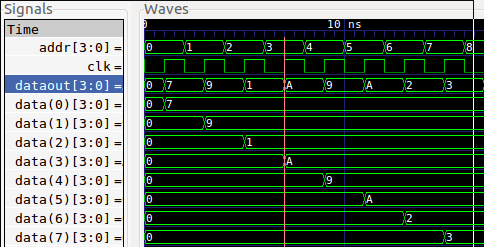
\includegraphics[width=9cm]{data/b1/bb507c-4cfa-404e-bf25-9e3a67321466/screenshot-20170328-102545.png}
\captionof{figure}{\label{fig:org86a5e18}
Lectura de RAM.}
\end{center}
\item Reset
\label{sec:orge5b378f}
\begin{center}
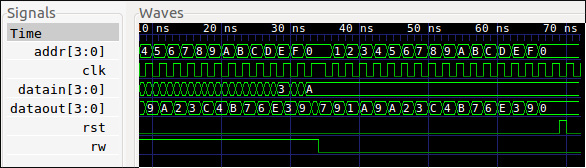
\includegraphics[width=9cm]{data/c9/deffbd-c88e-4470-adce-81f482ababd4/screenshot-20170405-000909.png}
\captionof{figure}{\label{fig:orgfeaf558}
Verificacion de reset en la memoria RAM}
\end{center}
\end{enumerate}


\subsection{{\bfseries\sffamily TODO} Ejemplo 3: CPU}
\label{sec:org105a531}

\subsection{{\bfseries\sffamily TODO} Ejemplo 4: Receptor UART}
\label{sec:org6887da7}

\bibliographystyle{plain}
\bibliography{bibliografia.bib}

\appendices
\section{Emacs}
\label{sec:orgc28221a}
\begin{center}
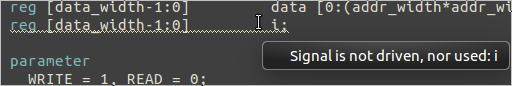
\includegraphics[width=10cm]{data/2d/d52799-180b-4118-8ce0-7e675d204eda/screenshot-20170327-121157.png}
\captionof{figure}{\label{fig:orgf9009ea}
La maquina virtual contiene un editor de texto llamado \texttt{Emacs}, este interactua directamente con \texttt{Verilator} mostrando mensajes de error.}
\end{center}

\begin{center}
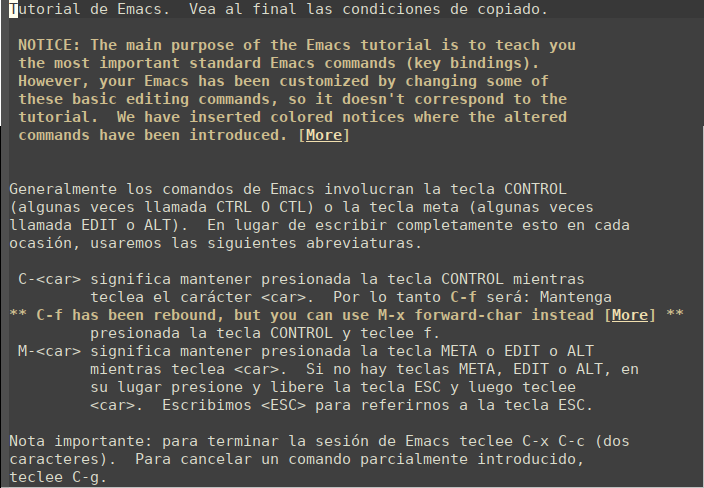
\includegraphics[width=10cm]{data/2d/d52799-180b-4118-8ce0-7e675d204eda/screenshot-20170327-121659.png}
\captionof{figure}{\label{fig:org1dbe502}
Se puede acceder al tutorial de emacs dentro de el presionando \texttt{Ctrl+h} y despues \texttt{t}.}
\end{center}
\end{document}